\documentclass[../delivery_hospital_report.tex]{subfiles}
\graphicspath{ {images/}{../images/} } 

\begin{document}
\chapter{Motivação}

Conforme o avanço de novas tecnologias vêm surgindo e se desenvolvendo, cada vez é mais comum encontrar-se equipamentos que não precisam da intervenção humana de forma constante para  a sua devida manipulação. Em um cenário hospitalar, ao qual o contato com equipamento está diretamente relacionado não somente a uma a comodidade, mas sim a disseminação de doenças, que colocam a vida de funcionários e paciente em risco.

Dessa forma, conforme o cenário pandêmico brasileiro se tornava mais evidente \cite{covid2020} e o número de mortes brasileiras por covid chegaram a números altos diante todo o cenário mundial \cite{mortes_covid21}, a construção de robô de entregas para um ambiente hospitalar, que não precise de intervenção humana para exercer suas funções básicas, com fins de diminuir contato e transição desnecessário pelo hospital se viu necessário hoje, e , sem dúvidas, indispensável para um futuro próximo.

\section{Primeiro Robô Hospitalar}

A Primeira versão do robô hospitalar era uma adaptação direta de um robô de entregas, que visava atuar, a princípio, dentro da cidade universitária da Universidade de São Paulo e arredores. Depois da adaptação, somente o lugar de atuação do robô foi alterado, ou seja, o robô que antes atuaria por toda a cidade universitária, atuaria somente dentro do Hospital Universitário.

\begin{figure}[h]
\centering
    \caption{1° Versão Robô Hospitalar}
    \centering % para centralizarmos a figura
    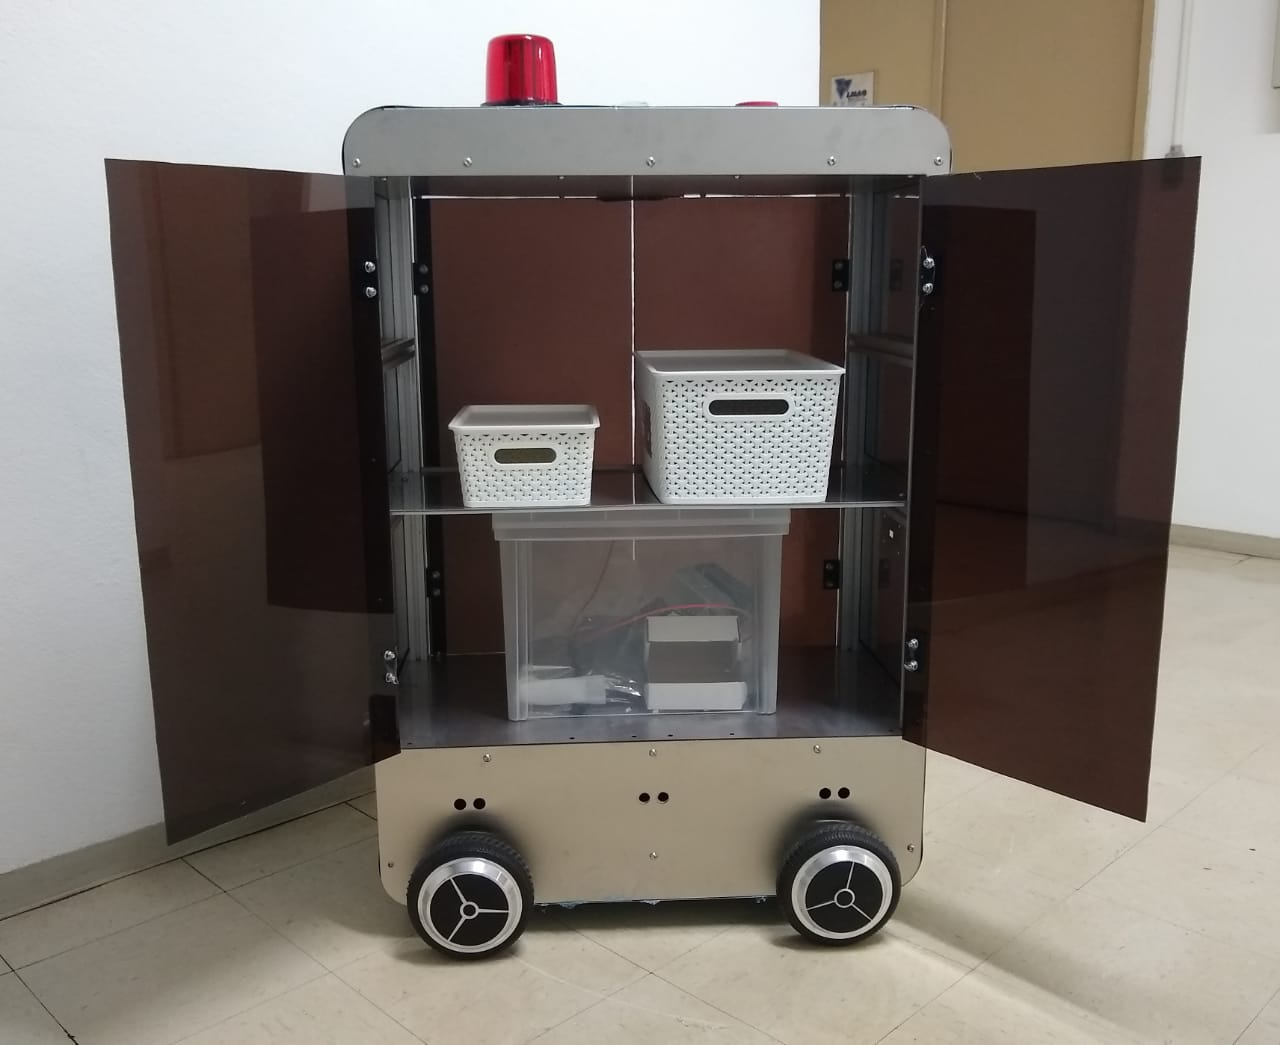
\includegraphics[width=10cm]{v1_robo_hospitalar.jpeg}
    \caption*{Fonte: Escola Politécnica da Universidade de São Paulo}
    \label{figura:1° Versão Robô Hospitalar}
\end{figure}

\subsection{Problemas}

À primeira vista, para um bom resultado do robô hospitalar, mostrava-se necessário somente a mudança do ambiente em que o robô estava imerso, mas que não o seu funcionamento lógico e físico. Porém, conforme teste e simulações foram feitas, alguns problemas importantes foram levantados em relação a essa primeira versão e a sua atuação no ambiente hospitalar.

Os problemas mais graves levantados, os mais alarmantes, eram em relação aos sistemas mecânicos e eletrônicos. Dentre esses problemas, destacava-se a estrutura do robô, que apresentava muitos parafusos, que além dificultar a montagem do robô, ainda facilitava no acúmulo de sujeira. Ademais, os sensores de distância alocados para o robô não eram precisos e de alto alcance, o que poderia gerar uma eventual colisão no hospital.

\section{Segundo Robô Hospitalar}

Após os problemas da primeira versão do robô hospitalar ficarem em evidência, a necessidade de realizar um novo projeto ficou plausível. Por conta disso, uma segunda versão do robô hospitalar, visando deixar o robô mais propício para o ambiente hospitalar, começou a ser produzida até o momento de escrita deste relatório. 

Por se tratar de um nova versão, a parte de hardware, software e mecânica do projeto foram reconstruídas como um todo. Nesse relatório de conclusão de Iniciação Científica vamos será abordado sobre toda a reconstrução até agosto de 2021 do robô hospitalar.

\begin{figure}[h]
\centering
    \caption{2° Versão Robô Hospitalar}
    \centering % para centralizarmos a figura
    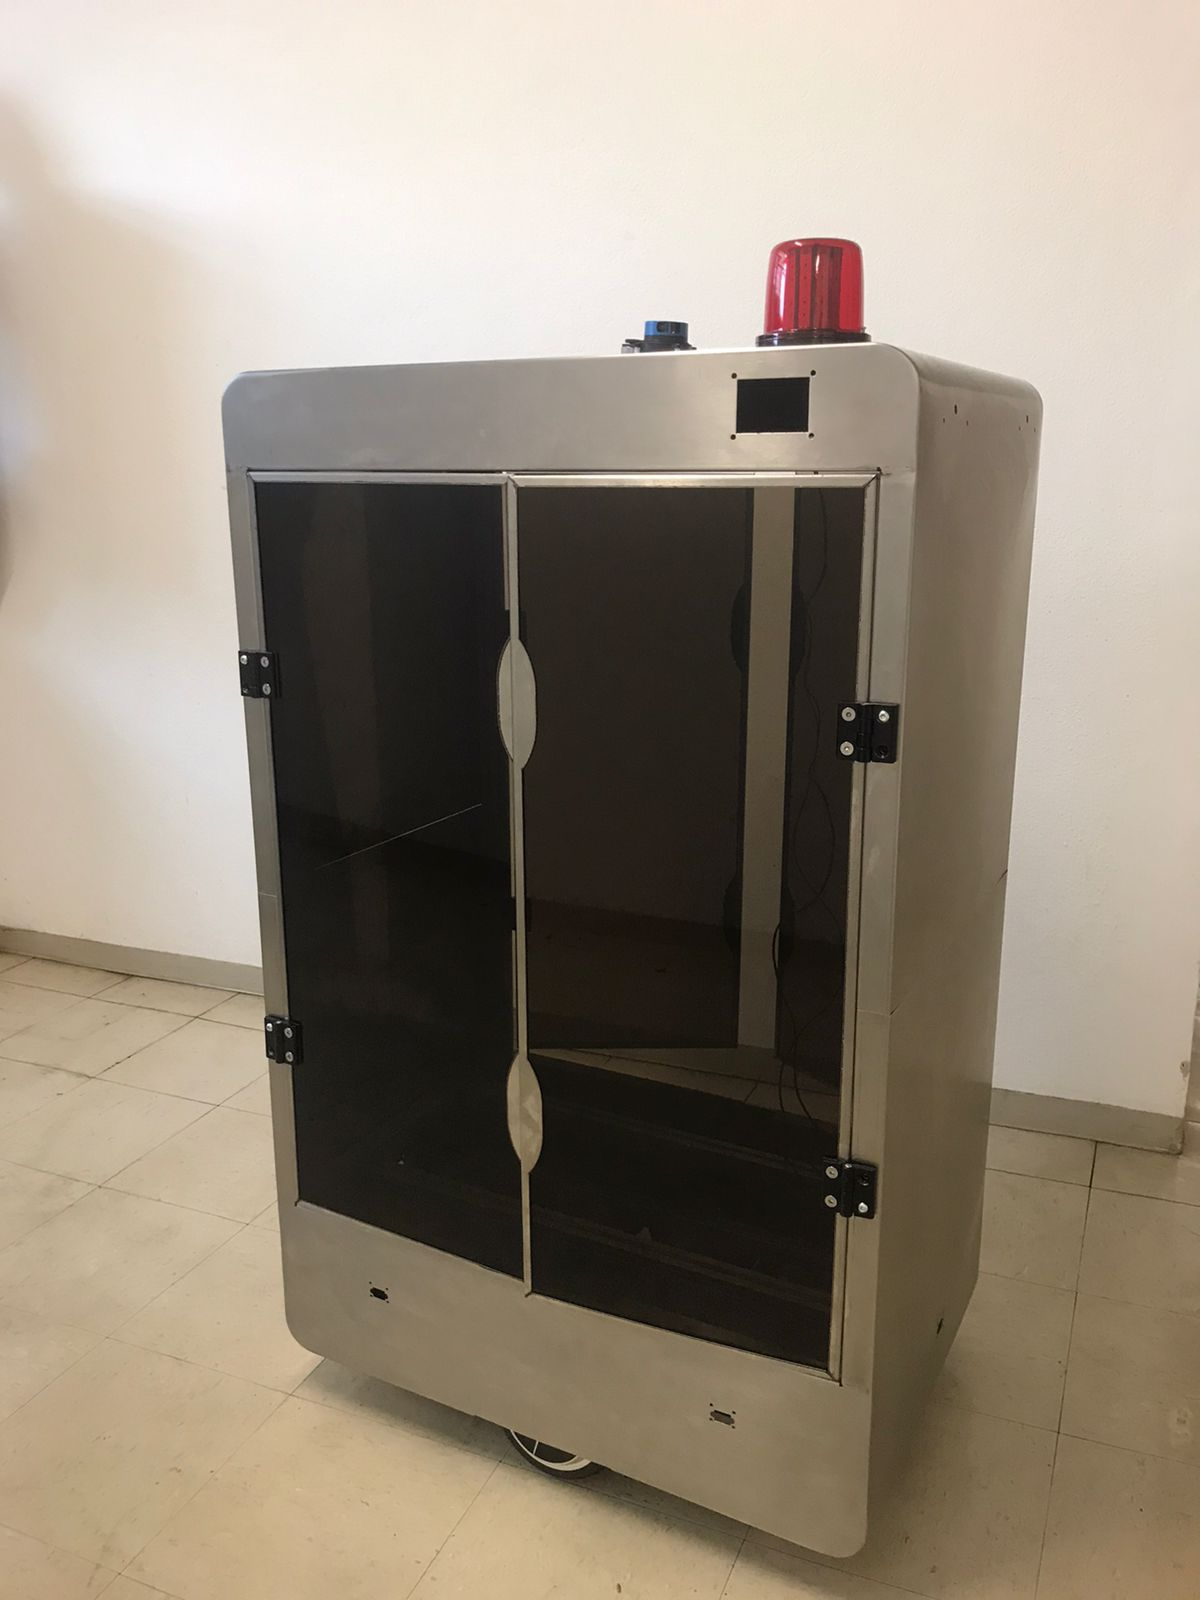
\includegraphics[width=10cm]{v2_robo_hospitalar.jpeg}
    \caption*{Fonte: Escola Politécnica da Universidade de São Paulo}
    \label{figura:1° Versão Robô Hospitalar}
\end{figure}

\end{document}